\documentclass{beamer}
%\documentclass[draft]{beamer}
%\documentclass[handout]{beamer}
\usepackage[latin1]{inputenc}
%\usepackage[ngerman]{babel}
\usepackage[english]{babel}
\usepackage{amssymb}

\usetheme{Boadilla}
\usefonttheme{professionalfonts}
\setbeamercovered{transparent}
\beamertemplatenavigationsymbolsempty
\setbeamertemplate{footline}[frame number]
\useinnertheme{rectangles}
\setbeamertemplate{blocks}[rounded][shadow=false]

\usepackage{enumerate} %% math
\usepackage{amsmath, amssymb} %%math
\usepackage{ulem} %%strike \sout{...}

\usepackage{tikz}
\usepackage{pgfpages}
\pgfpagesuselayout{resize to}[a4paper,border shrink=5mm,landscape]
\definecolor{orange}{RGB}{255,127,0}
\usepackage{listings}
\lstset{numbers=left,
	numberstyle=\footnotesize,
	numbersep=5pt,
	breaklines=true,
	showstringspaces=false,
	frame=l ,
	xleftmargin=15pt,
	xrightmargin=15pt,
	basicstyle=\ttfamily\small,
	stepnumber=1,
	keywordstyle=\color{blue},          % keyword style
  	commentstyle=\color{orange},       % comment style
%  	stringstyle=\color{green}         % string literal style
}
%Sprache Festelegen
\lstset{language=Python}
%\pgfpagesuselayout{two screens with lagging second} %% Pr�?sentation
%\pgfpagesuselayout{2 on 1}[a4paper,border shrink=5mm]
%\pgfpagesuselayout{4 on 1}[a4paper,border shrink=5mm, landscape]

%\pgfdeclareimage[width=.5\linewidth]{myimage}{images/myimage.png} % \pgfuseimage{myimage}

\pdfinfo{
  /Author (Robert M\"uller, Christian Lemke, Max Wagner, Mattes Wieben)
  /Title (Normalverteilung)
  /Subject (Normalverteilung)
  /Keywords (Normalverteilung)
}


\title{National and temporal divides in the themes of 19th century art}
\subtitle{Master Practical Course ``Data Analysis with Python''\\(WiSe 2016/17)}
%\titlegraphic{\includegraphics[width=0.15\textwidth]{./raspberry_pi_python_logo.png}}
\institute{
  Lehr- und Forschungseinheit f\"ur Programmier- und Modellierungssprachen\\
  Institut f\"ur Informatik\\
  Ludwig-Maximilians-Universit\"at M\"unchen\\[2em]
}

\author{Robert M\"uller, Christian Lemke, Max Wagner, Mattes Wieben}
\date{06. Februar 2017}


\begin{document}
%%%%%%%%%%%%%%%%%%%%%%%%%%%%%%%%%%%%%%%%%%%%%%%%%%%%%%%%%%%%%%%%%%%%%%%%%%%%%%%%
\begin{frame}
  \titlepage
\end{frame}


%%%%%%%%%%%%%%%%%%%%%%%%%%%%%%%%%%%%%%%%%%%%%%%%%%%%%%%%%%%%%%%%%%%%%%%%%%%%%%%%
\begin{frame}
  \frametitle{Agenda}
  \tableofcontents
\end{frame}

%%%%%%%%%%%%%%%%%%%%%%%%%%%%%%%%%%%%%%%%%%%%%%%%%%%%%%%%%%%%%%%%%%%%%%%%%%%%%%%%

\section{Clustering}
%%%%%%%%%%%%%%%%%%%%%%%%%%%%%%%%%%%%%%%%%%%%%%%%%%%%%%%%%%%%%%%%%%%%%%%%%%%%%%%%
\begin{frame}
  \frametitle{Clustering (1)}
  \begin{block}{}
    \begin{itemize}
      \item Sehr allgemeines Thema
			\item $\rightarrow$ Dictionary Ansatz zu speziell
      \item Ziel: Bildern verschiedene Themenbereiche zuordnen
    \end{itemize}
  \end{block}
	Schritt 1:\\
	Alle tags $t$ mit $P(t)> 0.4$ entfernen\\
	Bag of Words und Term Frequency - Inverse Document Frequency (TF-IDF)\\
	$bild_i=(tf\_idf(t_1),\dots, tf\_idf(t_n))$\\
\end{frame}

%%%%%%%%%%%%%%%%%%%%%%%%%%%%%%%%%%%%%%%%%%%%


\begin{frame}
  \frametitle{Clustering (2)}
	Schritt 2:\\
	Themen finden mittels Non-Negative-Matrix-Factorization\\
	$V\in\;{\rm I\!R}^{m\times n}_+ \quad \text{w\"ahle}\;k<<min(m,n)\;\text{mit}\;k\;\text{Anzahl der Themen}$
	$\text{finde}\;W\in\;{\rm I\!R}^{m\times k}_+\text{ und }H\in\;{\rm I\!R}^{k\times n}_+\text{ sodass }WH\approx V$
	\begin{figure}
    \centering
      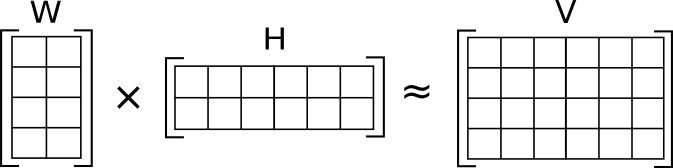
\includegraphics[width = 0.5\textwidth]{images/nmf.png}
  \end{figure}

  \begin{block}{Parameterwahl}
		\begin{itemize}
			\item $k=110$ durch Begutachtung der Ergebnisse f\"ur verschiedene $k$
			\item Ein Bild l\"asst sich nun \"uber 110 Themen beschreiben.
			\item Nach unseren Untersuchungen reichen die 4 Themen mit den h\"ochsten Werten um die Themen eines Bildes zu beschreiben
		\end{itemize}
  \end{block}
\end{frame}


\begin{frame}
  \frametitle{Clustering (3)}
	Beispiel Output :\\
	\textbf{Topic \#21:} \textit{uniform orden soldat kn\"opfe milit\"ar stiefel offizier sch\"arpe s\"abel degen general napoleon abzeichen epauletten soldaten}\\
	\textbf{Interpretation:} \textit{Uniform, Milit\"ar}\\
\end{frame}

\begin{frame}
  \frametitle{Clustering Beispiel}
	\begin{figure}
    \centering
      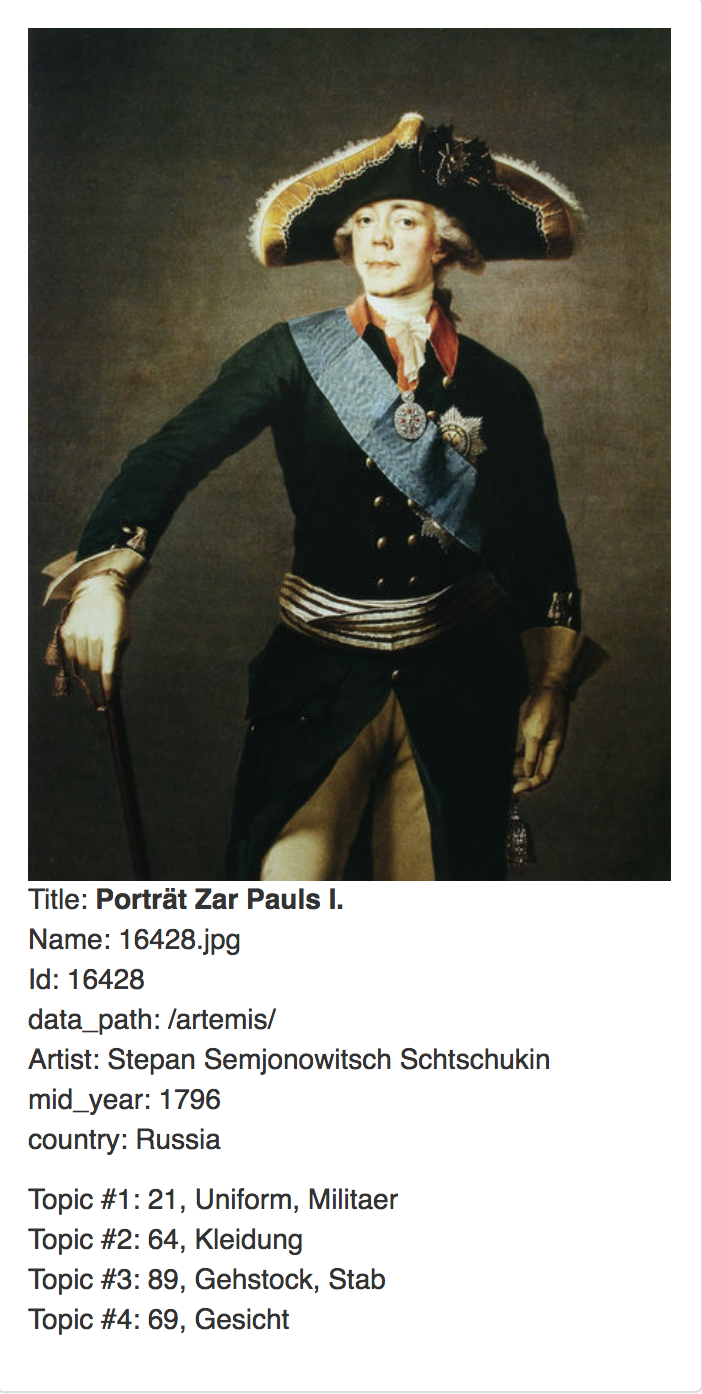
\includegraphics[width = 0.38\textwidth]{images/example_clustering_uniform.png}
  \end{figure}
\end{frame}

%%%%%%%%%%%%%%%%%%%%%%%%%%%%%%%%%%%%%%%%%%%%
\section{Analysetools}

\begin{frame}
\frametitle{Analysetools}
\centering
\textbf{Live Demo}
\end{frame}

%%%%%%%%%%%%%%%%%%%%%%%%%%%%%%%%%%%%%%%%%%%%
\section{Ergebnisse}

\begin{frame}
  \frametitle{Zeitliche und nationale Unterschiedlich bez\"uglich der Darstellung von Krieg}
  \begin{block}{}
    \begin{itemize}
      \item Krieg beliebtes Sujet in der bildenden Kunst (Annahme: ebenso im langen 19. Jhd.)\\
			\item Wichtigste Ereignisse: Franz\"osische Revolution, Koalitionskriege, Deutsche Revolutionen, 1. Weltkrieg\\
			\item Besonderer Fokus auf Frankreich
    \end{itemize}
  \end{block}
\end{frame}

\begin{frame}
  \frametitle{Zeitliche und nationale Unterschiedlich bez\"uglich der Darstellung von Krieg}
  \begin{block}{}
    \begin{itemize}
      \item Zwei Thesen zum Thema Krieg im langen 19. Jahrhundert:
			\begin{itemize}
				\item Franz\"osische Revolution als Vorbild weiterer Revolutionen in Europa\\
							Darstellung von Krieg Anfangs beliebt, danach steter Abfall\\
				\item Angst vor Krieg gegen Ende des langen 19. Jhd.\\
							Zahl der Bilder aus dem Cluster "Tod" nimmt zu
			\end{itemize}
    \end{itemize}
  \end{block}
	\begin{block}{}
		Topic clustering ergab f\"unf kriegsbezogene Cluster:
    \begin{itemize}
      \item Uniform
      \item R\"ustung
      \item Krieg
      \item Tod
      \item Feuer, Zerst\"orung
    \end{itemize}
  \end{block}
\end{frame}

\begin{frame}
\frametitle{War-topic relative H\"aufigkeit \"uber Zeit nach Nation}
  \begin{figure}
    \centering
      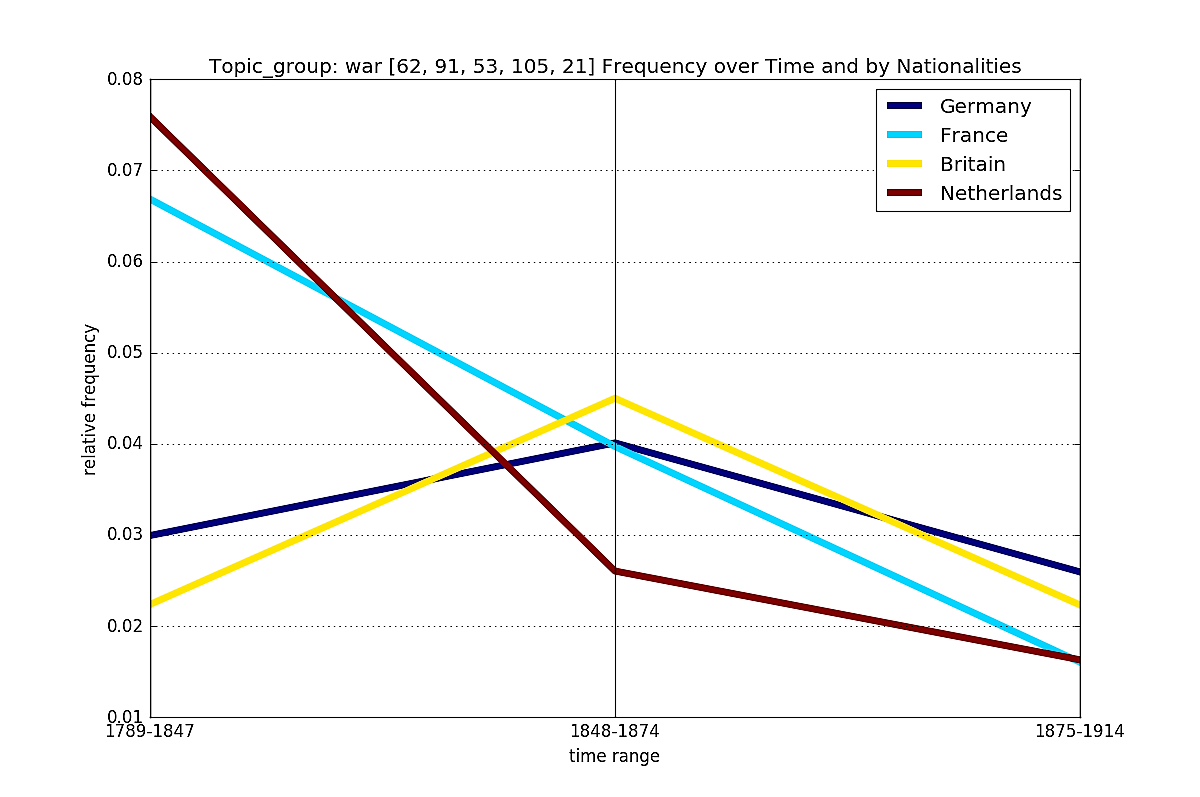
\includegraphics[width = \textwidth]{images/relFrequNations.png}
  \end{figure}
\end{frame}

\begin{frame}
\frametitle{Anteil der Kriegs-Cluster an Gesamtzahl der Bilder pro Zeitabschnitt}
  \begin{figure}
    \centering
      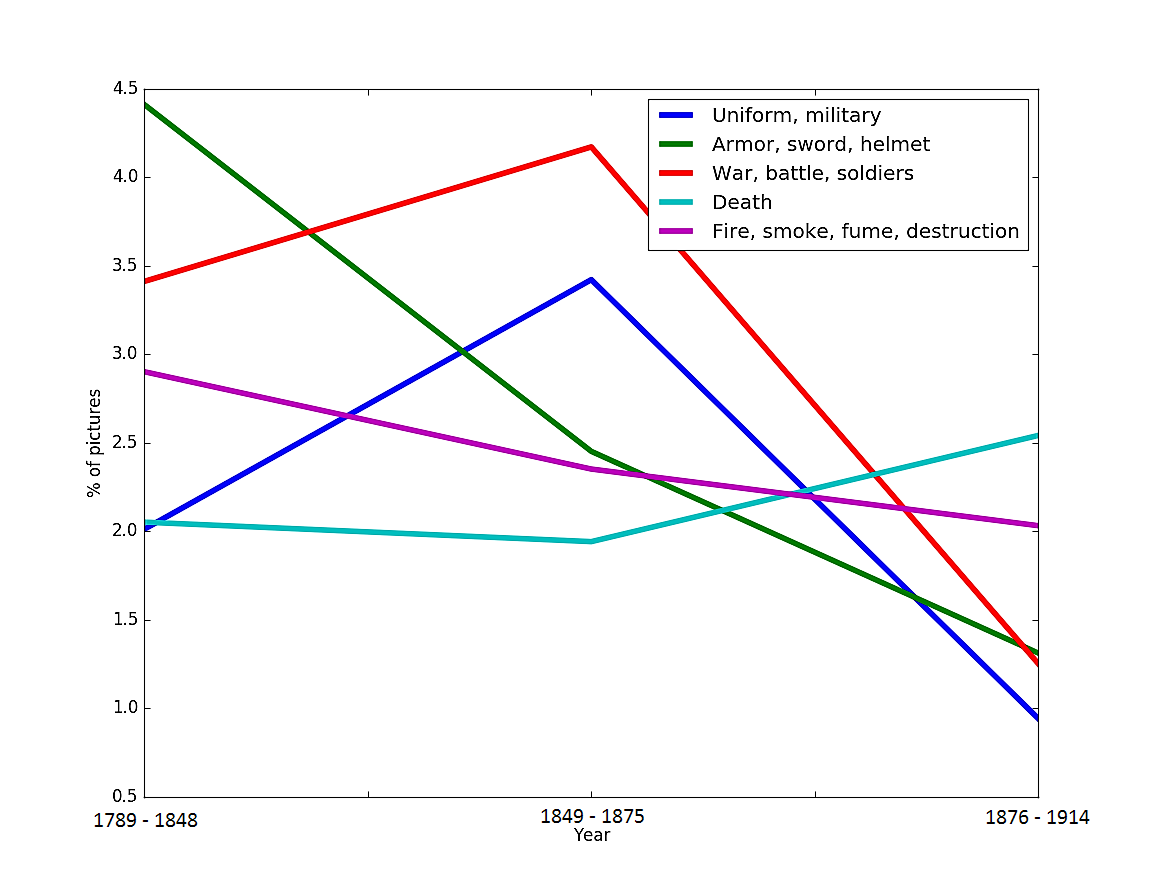
\includegraphics[width = 0.8\textwidth]{images/relDistTopics.png}
  \end{figure}
\end{frame}

\begin{frame}
  \frametitle{Religion}
    \begin{block}{}
    \begin{itemize}
      \item Die Kirche hat an gesellschaftlichem und politischen Einfluss verloren.
    \end{itemize}
  \end{block}
    \begin{figure}
    \centering
      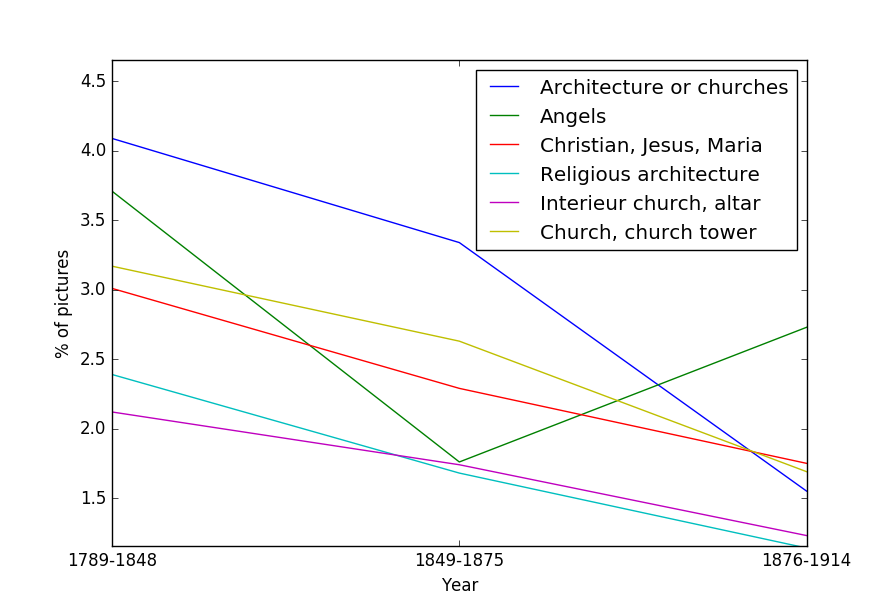
\includegraphics[width = 0.7\textwidth]{images/church2.png}
  \end{figure}
\end{frame}

\begin{frame}
  \frametitle{Religion}
    \begin{block}{}
    \begin{itemize}
      \item Die Kirche hat an gesellschaftlichem und politischen Einfluss verloren.
      \item Die S\"akularisierungswelle war in Frankreich am deutlichsten zu sp\"uren.
    \end{itemize}
  \end{block}
    \begin{figure}
    \centering
      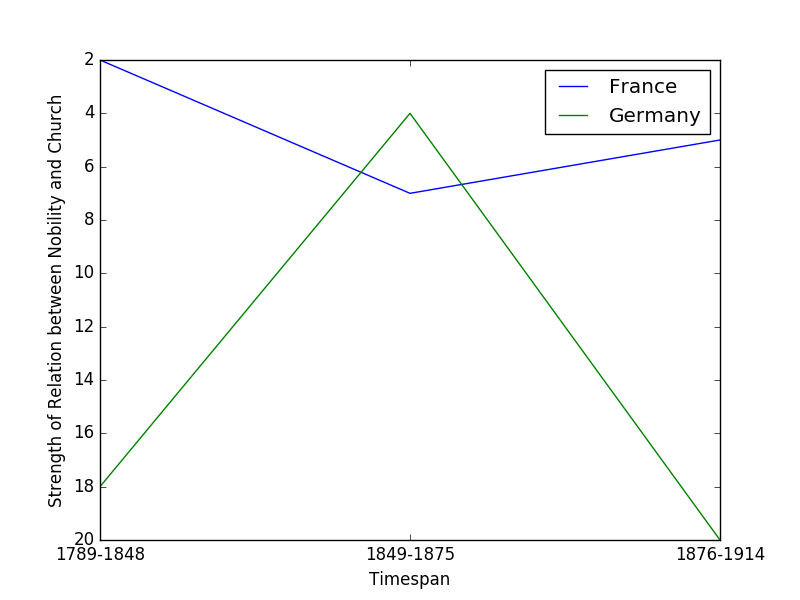
\includegraphics[width = 0.6\textwidth]{images/church3.png}
  \end{figure}
\end{frame}

\begin{frame}
  \frametitle{Religion}
    \begin{figure}
    \centering
      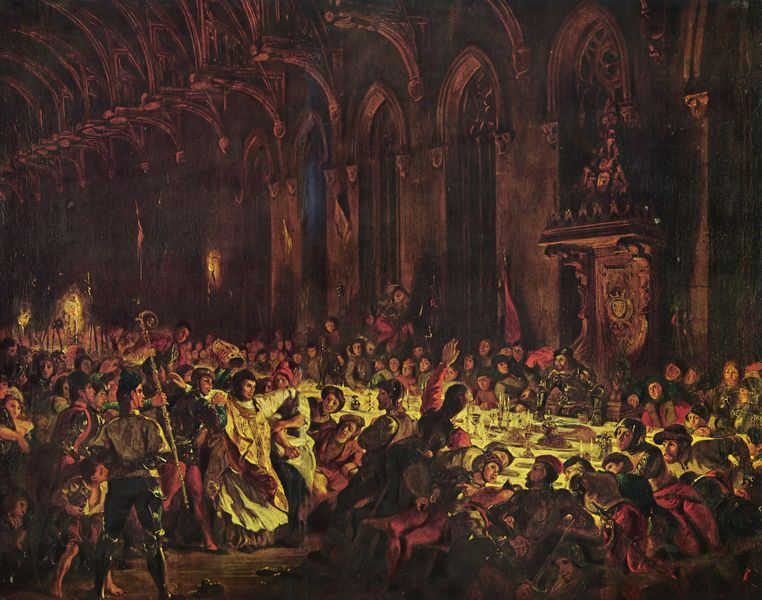
\includegraphics[width = 0.8\textwidth]{images/churchNobility_neu.jpg}
  \end{figure}
\end{frame}

\begin{frame}
  \frametitle{Religion}
    \begin{block}{}
    \begin{itemize}
      \item Die Kirche hat an gesellschaftlichem und politischen Einfluss verloren.
      \item Die S\"akularisierungswelle war in Frankreich am deutlichsten zu sp\"uren.
      \item Die Kirche ist sehr stark mit dem Tod verbunden.
    \end{itemize}
  \end{block}
    \begin{figure}
    \centering
      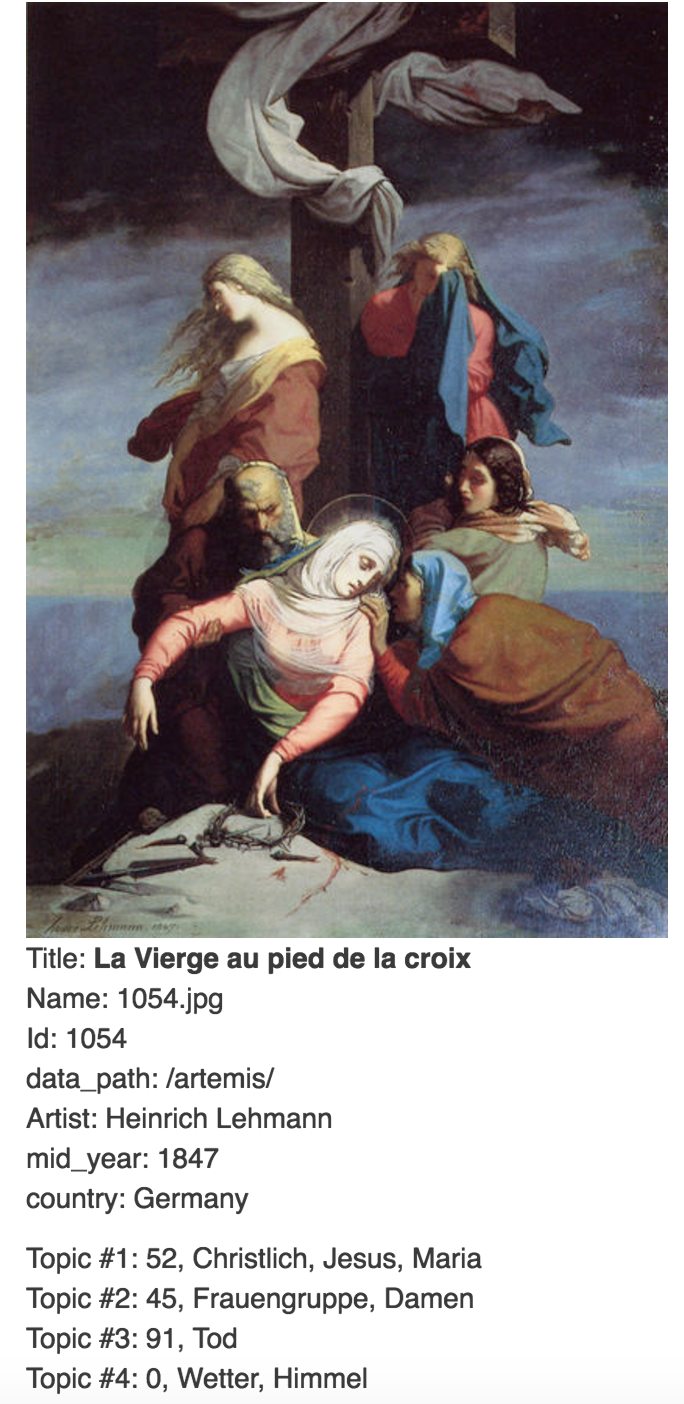
\includegraphics[width = 0.27\textwidth]{images/death_example.png}
  \end{figure}
\end{frame}

\begin{frame}
  \frametitle{Religion}
    \begin{block}{}
    \begin{itemize}
      \item Die Kirche hat an gesellschaftlichem und politischen Einfluss verloren.
      \item Die S\"akularisierungswelle war in Frankreich am deutlichsten zu sp\"uren.
      \item Die Kirche ist sehr stark mit dem Tod verbunden.
      \item Italienische Bilder hatten kaum kirchliche Relevanz.
    \end{itemize}
  \end{block}
    \begin{figure}
    \centering
      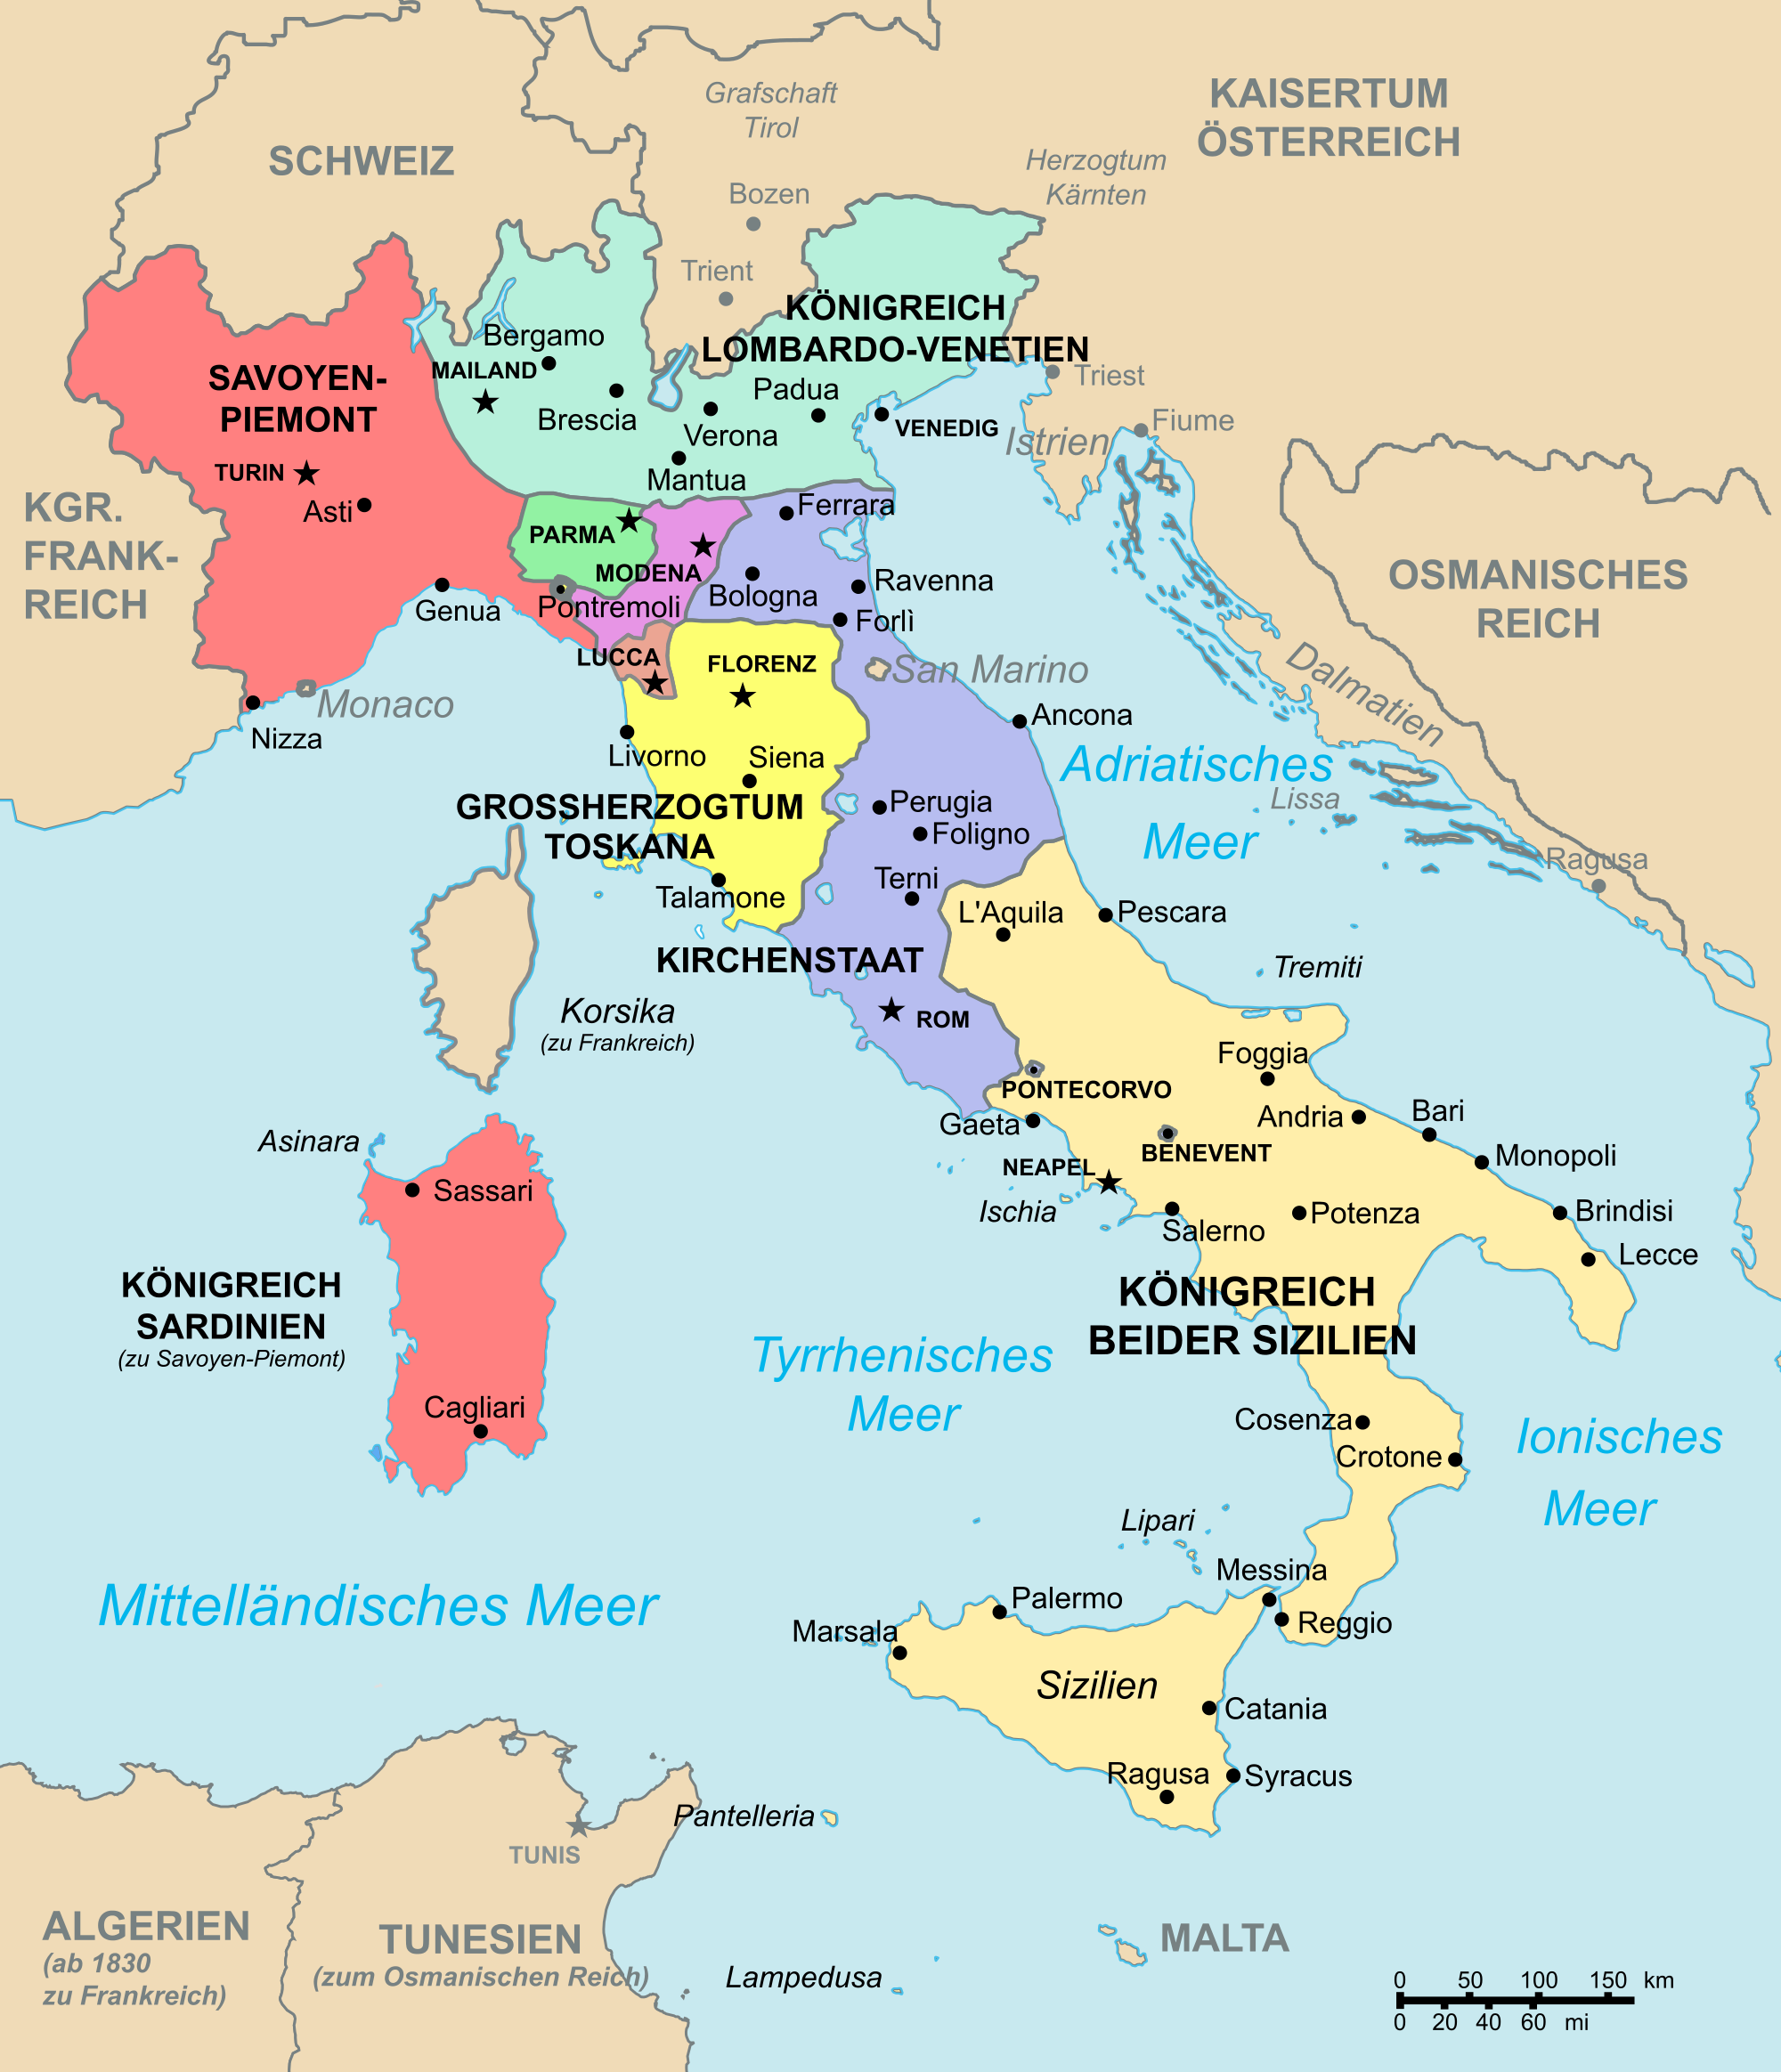
\includegraphics[width = 0.35\textwidth]{images/italien.png}
      \caption{Politische Lage Italien 1843 [1]}
  \end{figure}
\end{frame}

%%%%%%%%%%%%%%%%%%%%%%%%%%%%%%%%%%%%%%%%%%%%
\section{Ausblick und Zusammenfassung}

\begin{frame}
  \frametitle{Ausblick und Zusammenfassung}
  \begin{block}{}
    \begin{itemize}
      \item Das Clustering war sehr erfolgreich.
    \end{itemize}
  \end{block}
    \begin{figure}
    \centering
      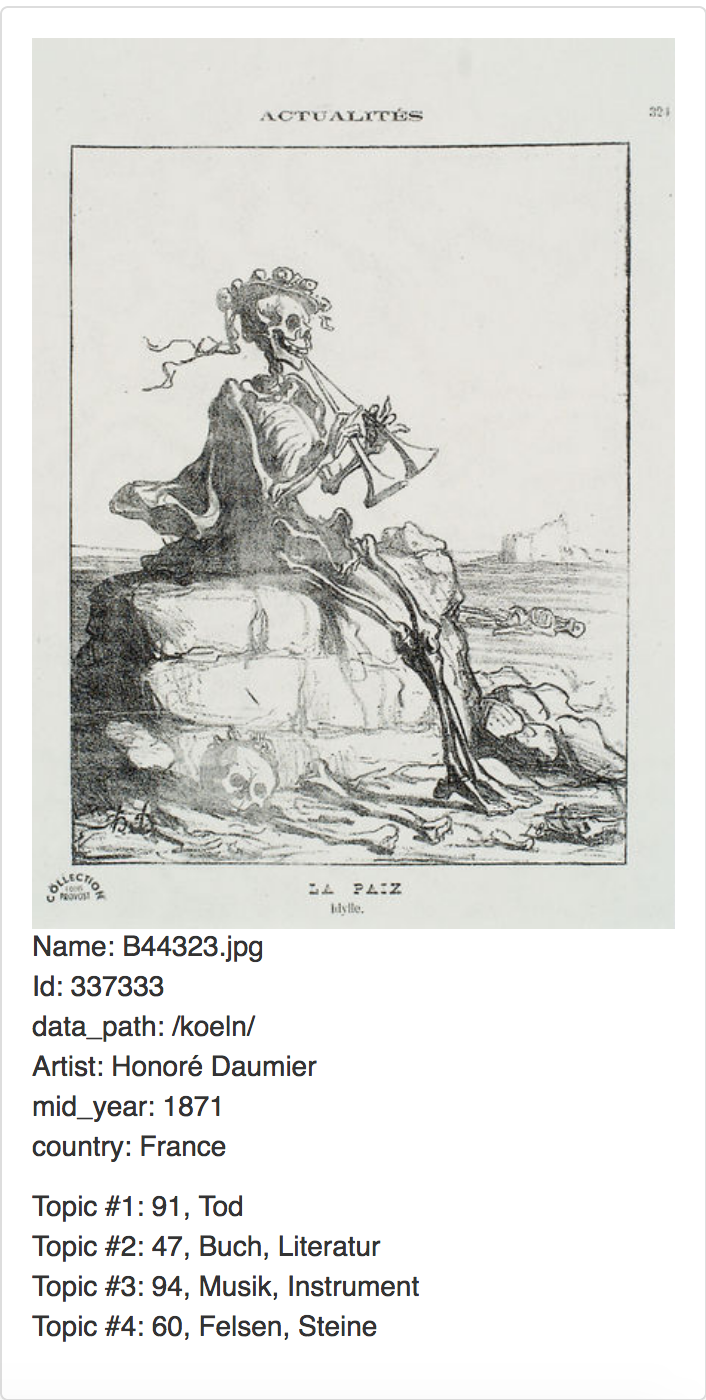
\includegraphics[width = 0.3\textwidth]{images/clustering_example_3.png}
  \end{figure}
\end{frame}

\begin{frame}
  \frametitle{Ausblick und Zusammenfassung}
  \begin{block}{}
    \begin{itemize}
      \item Das Clustering war sehr erfolgreich.
      \item Basierend darauf konnten hilfreiche Analyse-Tools, Matrizen und Graphen erstellt werden.
    \end{itemize}
  \end{block}
    \begin{figure}
    \centering
      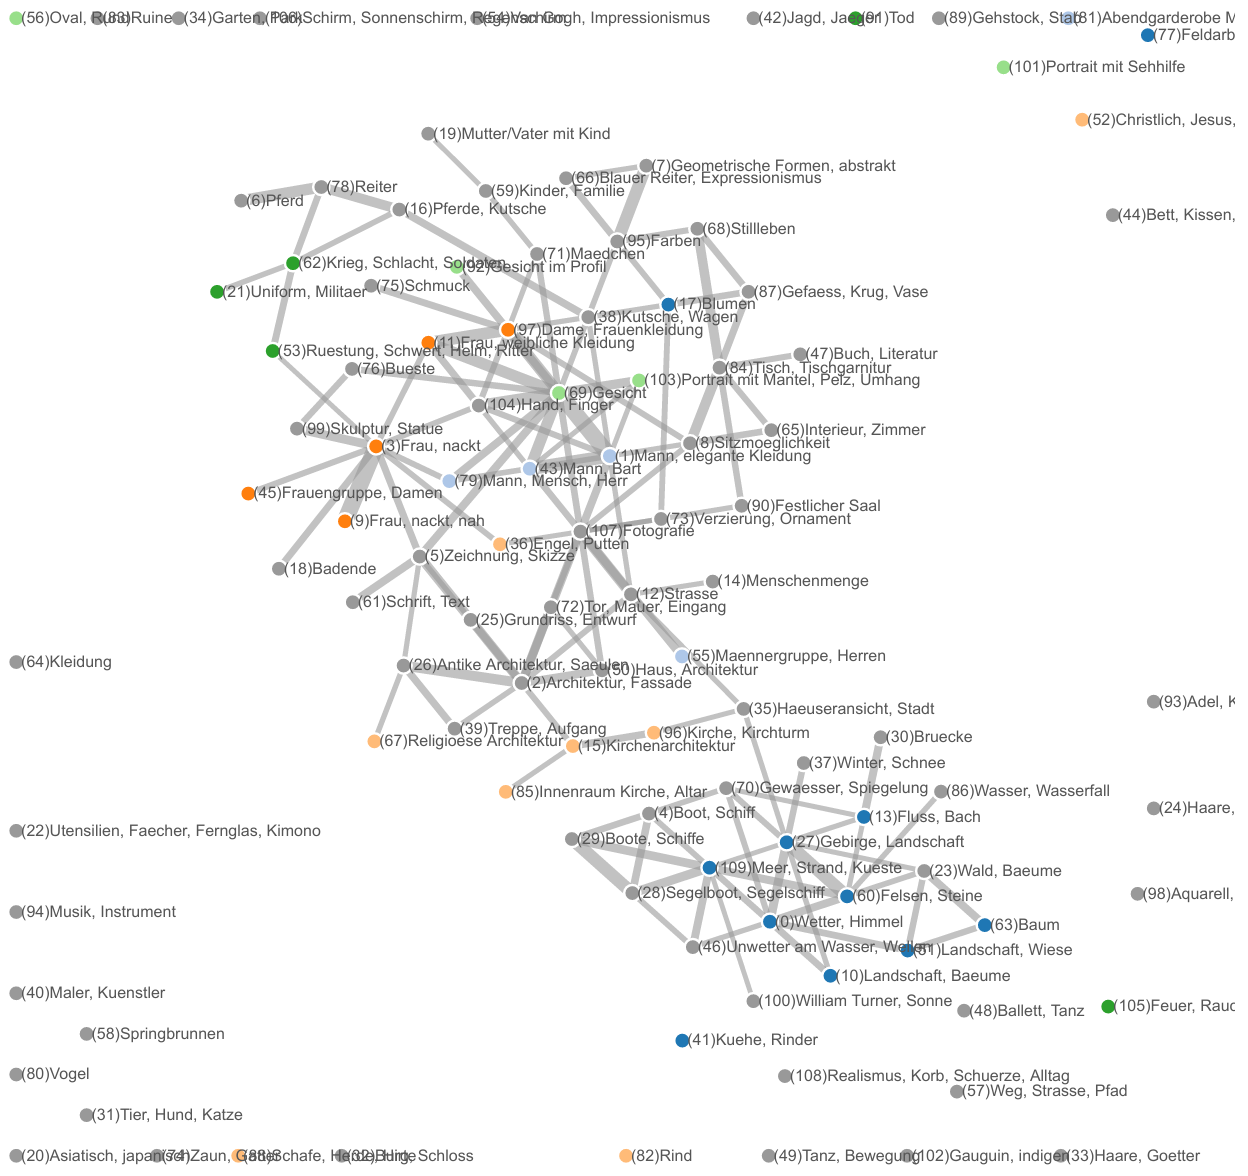
\includegraphics[width = 0.55\textwidth]{images/forcedgraph2.png}
  \end{figure}
\end{frame}

\begin{frame}
  \frametitle{Ausblick und Zusammenfassung}
  \begin{block}{}
    \begin{itemize}
      \item Das Clustering war sehr erfolgreich.
      \item Basierend darauf konnten hilfreiche Analyse-Tools, Matrizen und Graphen erstellt werden.
      \item Der abnehmende Einfluss der Kirche konnte gezeigt werden.
    \end{itemize}
  \end{block}
    \begin{figure}
    \centering
      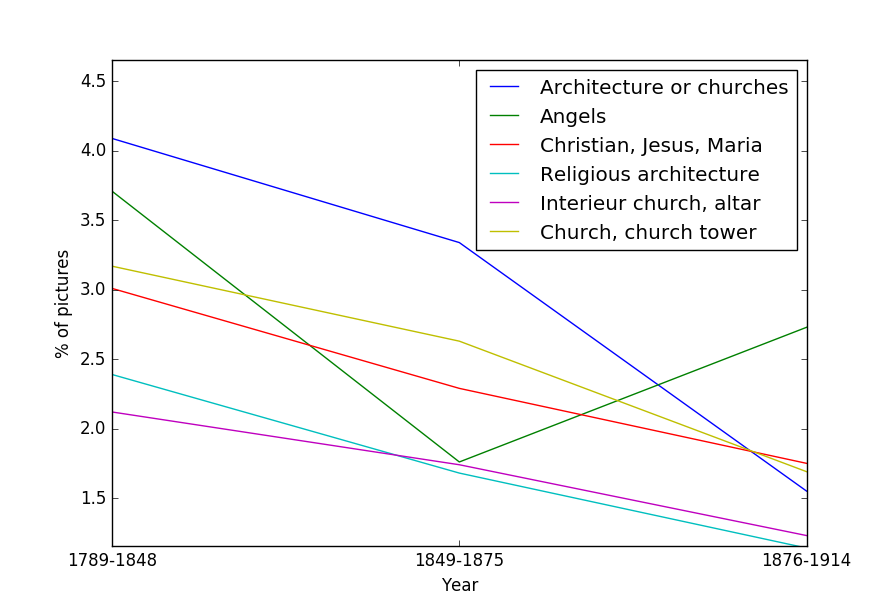
\includegraphics[width = 0.6\textwidth]{images/church2.png}
  \end{figure}
 \end{frame}

\begin{frame}
  \frametitle{Ausblick und Zusammenfassung}
  \begin{block}{}
    \begin{itemize}
      \item Das Clustering war sehr erfolgreich.
      \item Basierend darauf konnten hilfreiche Analyse-Tools, Matrizen und Graphen erstellt werden.
      \item Der abnehmende Einfluss der Kirche konnte gezeigt werden.
      \item Frankreichs Vorreiterrolle spiegelt sich auch in der Kunst wider.
    \end{itemize}
  \end{block}
    \begin{figure}
    \centering
      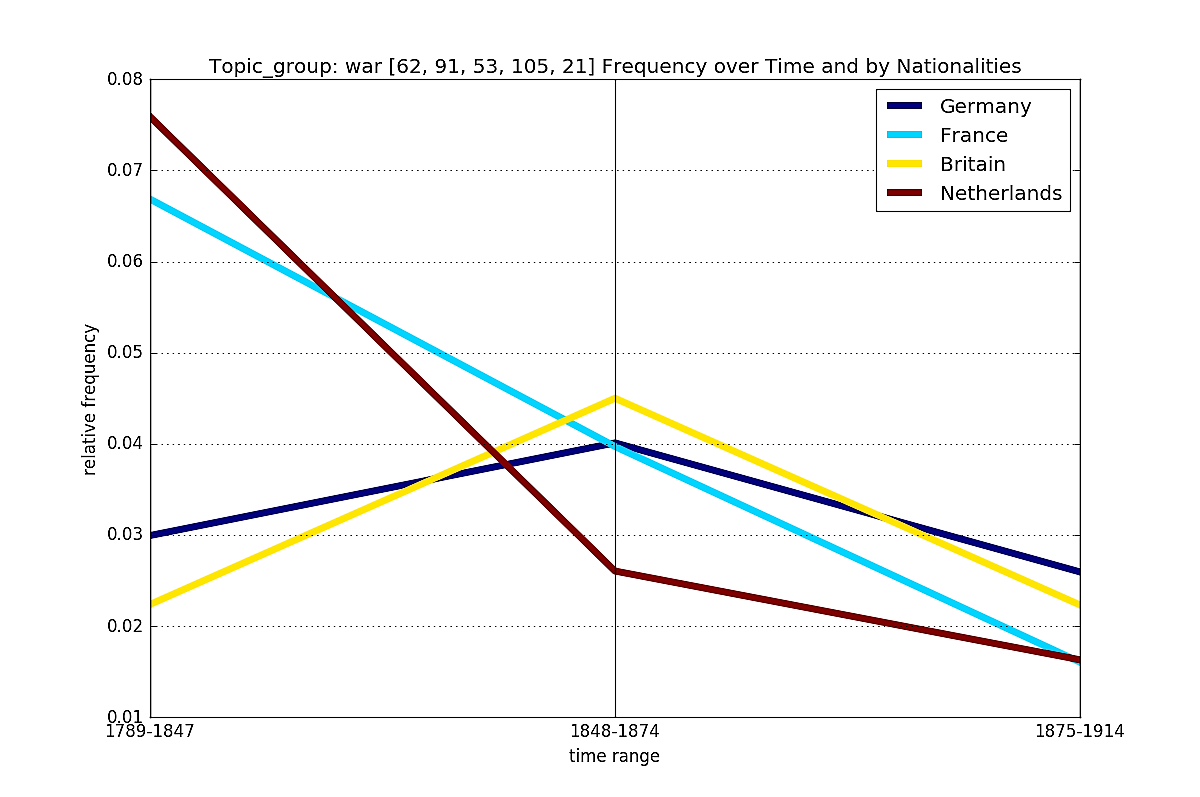
\includegraphics[width = 0.6\textwidth]{images/relFrequNations.png}
  \end{figure}\end{frame}

\begin{frame}
  \frametitle{Ausblick und Zusammenfassung}
  \begin{block}{}
    \begin{itemize}
      \item Das Clustering war sehr erfolgreich.
      \item Basierend darauf konnten hilfreiche Analyse-Tools, Matrizen und Graphen erstellt werden.
      \item Der abnehmende Einfluss der Kirche konnte gezeigt werden.
      \item Frankreichs Vorreiterrolle spiegelt sich auch in der Kunst wider.
      \item Es konnten weiterf\"uhrende Aufgaben aufgezeigt werden.
    \end{itemize}
  \end{block}
  $\Longrightarrow$ Flexible Zeitr\"aume\\
  $\Longrightarrow$ Gr\"o\ss{}erer (Italienischer) Datensatz
\end{frame}


%%%%%%%%%%%%%%%%%%%%%%%%%%%%%%%%%%%%%%%%%%%%
\section{Quellen}
\begin{frame}
  \frametitle{Quellen}
  \begin{block}{}
    \begin{itemize}
      \item Inhaltliche Quellen sind im Report aufgef�hrt.
    \end{itemize}
  \end{block}
  %[1]: https://upload.wikimedia.org/wikipedia/commons/thumb/d/de/Italy\_1843\_de.svg/2000px-Italy\_1843\_de.svg.png
  [1]: https://de.wikipedia.org/wiki/Italienische\_Unabh\"angigkeitskriege
\end{frame}



\end{document}
